\documentclass[journal, 8pt, twocolumn]{IEEEtran}

\usepackage{amsmath}
\usepackage{graphicx}

% FOR TABLE (according to table generated by ssconvert)
\def\inputGnumericTable{}
\usepackage[latin1]{inputenc}
\usepackage{color}
\usepackage{array}
\usepackage{longtable}
\usepackage{calc}
\usepackage{multirow}
\usepackage{hhline}
\usepackage{ifthen}
\usepackage{lscape}


\title{Assignment 3 \\}
\author{Abhishek Kumar\\AI21BTECH11003}

\begin{document}
	
	\maketitle
	
	\textbf{Question:}
	
	The following table gives the points scored by a kabaddi team in a series of match:
	\begin{table}[!htb]
		%%%%%%%%%%%%%%%%%%%%%%%%%%%%%%%%%%%%%%%%%%%%%%%%%%%%%%%%%%%%%%%%%%%%%%
%%                                                                  %%
%%  This is the header of a LaTeX2e file exported from Gnumeric.    %%
%%                                                                  %%
%%  This file can be compiled as it stands or included in another   %%
%%  LaTeX document. The table is based on the longtable package so  %%
%%  the longtable options (headers, footers...) can be set in the   %%
%%  preamble section below (see PRAMBLE).                           %%
%%                                                                  %%
%%  To include the file in another, the following two lines must be %%
%%  in the including file:                                          %%
%%        \def\inputGnumericTable{}                                 %%
%%  at the beginning of the file and:                               %%
%%        \input{name-of-this-file.tex}                             %%
%%  where the table is to be placed. Note also that the including   %%
%%  file must use the following packages for the table to be        %%
%%  rendered correctly:                                             %%
%%    \usepackage[latin1]{inputenc}                                 %%
%%    \usepackage{color}                                            %%
%%    \usepackage{array}                                            %%
%%    \usepackage{longtable}                                        %%
%%    \usepackage{calc}                                             %%
%%    \usepackage{multirow}                                         %%
%%    \usepackage{hhline}                                           %%
%%    \usepackage{ifthen}                                           %%
%%  optionally (for landscape tables embedded in another document): %%
%%    \usepackage{lscape}                                           %%
%%                                                                  %%
%%%%%%%%%%%%%%%%%%%%%%%%%%%%%%%%%%%%%%%%%%%%%%%%%%%%%%%%%%%%%%%%%%%%%%



%%  This section checks if we are begin input into another file or  %%
%%  the file will be compiled alone. First use a macro taken from   %%
%%  the TeXbook ex 7.7 (suggestion of Han-Wen Nienhuys).            %%
\def\ifundefined#1{\expandafter\ifx\csname#1\endcsname\relax}


%%  Check for the \def token for inputed files. If it is not        %%
%%  defined, the file will be processed as a standalone and the     %%
%%  preamble will be used.                                          %%
\ifundefined{inputGnumericTable}

%%  We must be able to close or not the document at the end.        %%
\def\gnumericTableEnd{\end{document}}


%%%%%%%%%%%%%%%%%%%%%%%%%%%%%%%%%%%%%%%%%%%%%%%%%%%%%%%%%%%%%%%%%%%%%%
%%                                                                  %%
%%  This is the PREAMBLE. Change these values to get the right      %%
%%  paper size and other niceties.                                  %%
%%                                                                  %%
%%%%%%%%%%%%%%%%%%%%%%%%%%%%%%%%%%%%%%%%%%%%%%%%%%%%%%%%%%%%%%%%%%%%%%

\documentclass[12pt%
%,landscape%
]{report}
\usepackage[latin1]{inputenc}
\usepackage{fullpage}
\usepackage{color}
\usepackage{array}
\usepackage{longtable}
\usepackage{calc}
\usepackage{multirow}
\usepackage{hhline}
\usepackage{ifthen}

\begin{document}


%%  End of the preamble for the standalone. The next section is for %%
%%  documents which are included into other LaTeX2e files.          %%
\else

%%  We are not a stand alone document. For a regular table, we will %%
%%  have no preamble and only define the closing to mean nothing.   %%
\def\gnumericTableEnd{}

%%  If we want landscape mode in an embedded document, comment out  %%
%%  the line above and uncomment the two below. The table will      %%
%%  begin on a new page and run in landscape mode.                  %%
%       \def\gnumericTableEnd{\end{landscape}}
%       \begin{landscape}


%%  End of the else clause for this file being \input.              %%
\fi

%%%%%%%%%%%%%%%%%%%%%%%%%%%%%%%%%%%%%%%%%%%%%%%%%%%%%%%%%%%%%%%%%%%%%%
%%                                                                  %%
%%  The rest is the gnumeric table, except for the closing          %%
%%  statement. Changes below will alter the table's appearance.     %%
%%                                                                  %%
%%%%%%%%%%%%%%%%%%%%%%%%%%%%%%%%%%%%%%%%%%%%%%%%%%%%%%%%%%%%%%%%%%%%%%

\providecommand{\gnumericmathit}[1]{#1} 
%%  Uncomment the next line if you would like your numbers to be in %%
%%  italics if they are italizised in the gnumeric table.           %%
%\renewcommand{\gnumericmathit}[1]{\mathit{#1}}
\providecommand{\gnumericPB}[1]%
{\let\gnumericTemp=\\#1\let\\=\gnumericTemp\hspace{0pt}}
\ifundefined{gnumericTableWidthDefined}
\newlength{\gnumericTableWidth}
\newlength{\gnumericTableWidthComplete}
\newlength{\gnumericMultiRowLength}
\global\def\gnumericTableWidthDefined{}
\fi
%% The following setting protects this code from babel shorthands.  %%
\ifthenelse{\isundefined{\languageshorthands}}{}{\languageshorthands{english}}
%%  The default table format retains the relative column widths of  %%
%%  gnumeric. They can easily be changed to c, r or l. In that case %%
%%  you may want to comment out the next line and uncomment the one %%
%%  thereafter                                                      %%
\providecommand\gnumbox{\makebox[0pt]}
%%\providecommand\gnumbox[1][]{\makebox}

%% to adjust positions in multirow situations                       %%
\setlength{\bigstrutjot}{\jot}
\setlength{\extrarowheight}{\doublerulesep}

%%  The \setlongtables command keeps column widths the same across  %%
%%  pages. Simply comment out next line for varying column widths.  %%
\setlongtables

\setlength\gnumericTableWidth{%
	53pt+%
	53pt+%
	53pt+%
	53pt+%
	53pt+%
	0pt}
\def\gumericNumCols{5}
\setlength\gnumericTableWidthComplete{\gnumericTableWidth+%
	\tabcolsep*\gumericNumCols*2+\arrayrulewidth*\gumericNumCols}
\ifthenelse{\lengthtest{\gnumericTableWidthComplete > \linewidth}}%
{\def\gnumericScale{1*\ratio{\linewidth-%
			\tabcolsep*\gumericNumCols*2-%
			\arrayrulewidth*\gumericNumCols}%
		{\gnumericTableWidth}}}%
{\def\gnumericScale{1}}

%%%%%%%%%%%%%%%%%%%%%%%%%%%%%%%%%%%%%%%%%%%%%%%%%%%%%%%%%%%%%%%%%%%%%%
%%                                                                  %%
%% The following are the widths of the various columns. We are      %%
%% defining them here because then they are easier to change.       %%
%% Depending on the cell formats we may use them more than once.    %%
%%                                                                  %%
%%%%%%%%%%%%%%%%%%%%%%%%%%%%%%%%%%%%%%%%%%%%%%%%%%%%%%%%%%%%%%%%%%%%%%

\ifthenelse{\isundefined{\gnumericColA}}{\newlength{\gnumericColA}}{}\settowidth{\gnumericColA}{\begin{tabular}{@{}p{53pt*\gnumericScale}@{}}x\end{tabular}}
\ifthenelse{\isundefined{\gnumericColB}}{\newlength{\gnumericColB}}{}\settowidth{\gnumericColB}{\begin{tabular}{@{}p{53pt*\gnumericScale}@{}}x\end{tabular}}
\ifthenelse{\isundefined{\gnumericColC}}{\newlength{\gnumericColC}}{}\settowidth{\gnumericColC}{\begin{tabular}{@{}p{53pt*\gnumericScale}@{}}x\end{tabular}}
\ifthenelse{\isundefined{\gnumericColD}}{\newlength{\gnumericColD}}{}\settowidth{\gnumericColD}{\begin{tabular}{@{}p{53pt*\gnumericScale}@{}}x\end{tabular}}
\ifthenelse{\isundefined{\gnumericColE}}{\newlength{\gnumericColE}}{}\settowidth{\gnumericColE}{\begin{tabular}{@{}p{53pt*\gnumericScale}@{}}x\end{tabular}}

\begin{longtable}[c]{%
		b{\gnumericColA}%
		b{\gnumericColB}%
		b{\gnumericColC}%
		b{\gnumericColD}%
		b{\gnumericColE}%
	}
	
	%%%%%%%%%%%%%%%%%%%%%%%%%%%%%%%%%%%%%%%%%%%%%%%%%%%%%%%%%%%%%%%%%%%%%%
	%%  The longtable options. (Caption, headers... see Goosens, p.124) %%
	%	\caption{The Table Caption.}             \\	%
	% \hline	% Across the top of the table.
	%%  The rest of these options are table rows which are placed on    %%
	%%  the first, last or every page. Use \multicolumn if you want.    %%
	
	%%  Header for the first page.                                      %%
	%	\multicolumn{5}{c}{The First Header} \\ \hline 
	%	\multicolumn{1}{c}{colTag}	%Column 1
	%	&\multicolumn{1}{c}{colTag}	%Column 2
	%	&\multicolumn{1}{c}{colTag}	%Column 3
	%	&\multicolumn{1}{c}{colTag}	%Column 4
	%	&\multicolumn{1}{c}{colTag}	\\ \hline %Last column
	%	\endfirsthead
	
	%%  The running header definition.                                  %%
	%	\hline
	%	\multicolumn{5}{l}{\ldots\small\slshape continued} \\ \hline
	%	\multicolumn{1}{c}{colTag}	%Column 1
	%	&\multicolumn{1}{c}{colTag}	%Column 2
	%	&\multicolumn{1}{c}{colTag}	%Column 3
	%	&\multicolumn{1}{c}{colTag}	%Column 4
	%	&\multicolumn{1}{c}{colTag}	\\ \hline %Last column
	%	\endhead
	
	%%  The running footer definition.                                  %%
	%	\hline
	%	\multicolumn{5}{r}{\small\slshape continued\ldots} \\
	%	\endfoot
	
	%%  The ending footer definition.                                   %%
	%	\multicolumn{5}{c}{That's all folks} \\ \hline 
	%	\endlastfoot
	%%%%%%%%%%%%%%%%%%%%%%%%%%%%%%%%%%%%%%%%%%%%%%%%%%%%%%%%%%%%%%%%%%%%%%
	
	\hhline{|--|--~}
	\multicolumn{2}{|p{	\gnumericColA+%
			\gnumericColB+%
			\tabcolsep*2*1}|}%
	{\gnumericPB{\centering}\gnumbox{\textbf{(X)}}}
	&\multicolumn{2}{p{	\gnumericColC+%
			\gnumericColD+%
			\tabcolsep*2*1}|}%
	{\gnumericPB{\centering}\gnumbox{\textbf{Match No.}}}
	&
	\\
	\hhline{|--|--~}
	\multicolumn{2}{|p{	\gnumericColA+%
			\gnumericColB+%
			\tabcolsep*2*1}|}%
	{\gnumericPB{\centering}\gnumbox{\textbf{Points scored by team}}}
	&\multicolumn{2}{p{	\gnumericColC+%
			\gnumericColD+%
			\tabcolsep*2*1}|}%
	{\gnumericPB{\centering}\gnumbox{\textbf{Match No.}}}
	&
	\\
	
	\hhline{|--|--~}
	\multicolumn{2}{|p{\gnumericColA}|}%
	{\gnumericPB{\centering}\gnumbox[l]{17}}
	&\multicolumn{2}{p{\gnumericColB}|}%
	{\gnumericPB{\centering}\gnumbox[r]{1}}
	&
	
	
	\\
	\hhline{|--|--~}
	\multicolumn{2}{|p{\gnumericColA}|}%
	{\gnumericPB{\centering}\gnumbox[l]{2}}
	&\multicolumn{2}{p{\gnumericColB}|}%
	{\gnumericPB{\centering}\gnumbox[r]{2}}
	&
	
	
	\\
	\hhline{|--|--~}
	\multicolumn{2}{|p{\gnumericColA}|}%
	{\gnumericPB{\centering}\gnumbox[l]{7}}
	&\multicolumn{2}{p{\gnumericColB}|}%
	{\gnumericPB{\centering}\gnumbox[r]{3}}
	&
	
	
	\\
	\hhline{|--|--~}
	\multicolumn{2}{|p{\gnumericColA}|}%
	{\gnumericPB{\centering}\gnumbox[l]{27}}
	&\multicolumn{2}{p{\gnumericColB}|}%
	{\gnumericPB{\centering}\gnumbox[r]{4}}
	&
	
	
	\\
	\hhline{|--|--~}
	\multicolumn{2}{|p{\gnumericColA}|}%
	{\gnumericPB{\centering}\gnumbox[l]{15}}
	&\multicolumn{2}{p{\gnumericColB}|}%
	{\gnumericPB{\centering}\gnumbox[r]{5}}
	&
	
	
	\\
	\hhline{|--|--~}
	\multicolumn{2}{|p{\gnumericColA}|}%
	{\gnumericPB{\centering}\gnumbox[l]{5}}
	&\multicolumn{2}{p{\gnumericColB}|}%
	{\gnumericPB{\centering}\gnumbox[r]{6}}
	&
	
	
	\\
	\hhline{|--|--~}
	\multicolumn{2}{|p{\gnumericColA}|}%
	{\gnumericPB{\centering}\gnumbox[l]{14}}
	&\multicolumn{2}{p{\gnumericColB}|}%
	{\gnumericPB{\centering}\gnumbox[r]{7}}
	&
	
	
	\\
	\hhline{|--|--~}
	\multicolumn{2}{|p{\gnumericColA}|}%
	{\gnumericPB{\centering}\gnumbox[l]{8}}
	&\multicolumn{2}{p{\gnumericColB}|}%
	{\gnumericPB{\centering}\gnumbox[r]{8}}
	&
	
	
	\\
	\hhline{|--|--~}
	\multicolumn{2}{|p{\gnumericColA}|}%
	{\gnumericPB{\centering}\gnumbox[l]{10}}
	&\multicolumn{2}{p{\gnumericColB}|}%
	{\gnumericPB{\centering}\gnumbox[r]{9}}
	&
	
	
	\\
	\hhline{|--|--~}
	\multicolumn{2}{|p{\gnumericColA}|}%
	{\gnumericPB{\centering}\gnumbox[l]{24}}
	&\multicolumn{2}{p{\gnumericColB}|}%
	{\gnumericPB{\centering}\gnumbox[r]{10}}
	&
	
	
	\\
	\hhline{|--|--~}
	\multicolumn{2}{|p{\gnumericColA}|}%
	{\gnumericPB{\centering}\gnumbox[l]{48}}
	&\multicolumn{2}{p{\gnumericColB}|}%
	{\gnumericPB{\centering}\gnumbox[r]{11}}
	&
	
	
	\\
	\hhline{|--|--~}
	\multicolumn{2}{|p{\gnumericColA}|}%
	{\gnumericPB{\centering}\gnumbox[l]{10}}
	&\multicolumn{2}{p{\gnumericColB}|}%
	{\gnumericPB{\centering}\gnumbox[r]{12}}
	&
	
	
	\\
	\hhline{|--|--~}
	\multicolumn{2}{|p{\gnumericColA}|}%
	{\gnumericPB{\centering}\gnumbox[l]{8}}
	&\multicolumn{2}{p{\gnumericColB}|}%
	{\gnumericPB{\centering}\gnumbox[r]{13}}
	&
	
	
	\\
	\hhline{|--|--~}
	\multicolumn{2}{|p{\gnumericColA}|}%
	{\gnumericPB{\centering}\gnumbox[l]{7}}
	&\multicolumn{2}{p{\gnumericColB}|}%
	{\gnumericPB{\centering}\gnumbox[r]{14}}
	&
	
	
	\\
	\hhline{|--|--~}
	\multicolumn{2}{|p{\gnumericColA}|}%
	{\gnumericPB{\centering}\gnumbox[l]{18}}
	&\multicolumn{2}{p{\gnumericColB}|}%
	{\gnumericPB{\centering}\gnumbox[r]{15}}
	&
	
	
	\\
	\hhline{|--|--~}
	\multicolumn{2}{|p{\gnumericColA}|}%
	{\gnumericPB{\centering}\gnumbox[l]{28}}
	&\multicolumn{2}{p{\gnumericColB}|}%
	{\gnumericPB{\centering}\gnumbox[r]{16}}
	&
	
	
	
	\\
	\hhline{|-|-|-|-|~}
\end{longtable}

\ifthenelse{\isundefined{\languageshorthands}}{}{\languageshorthands{\languagename}}
\gnumericTableEnd
		\caption{}
		\label{table:data}
	\end{table}
	
	
	find median of the points scored by team.
	
	\textbf{Solution:}
	
	Firstly we arrange the different scores/points in ascending order.
	
	\begin{table}[!htb]
		%%%%%%%%%%%%%%%%%%%%%%%%%%%%%%%%%%%%%%%%%%%%%%%%%%%%%%%%%%%%%%%%%%%%%%
%%                                                                  %%
%%  This is the header of a LaTeX2e file exported from Gnumeric.    %%
%%                                                                  %%
%%  This file can be compiled as it stands or included in another   %%
%%  LaTeX document. The table is based on the longtable package so  %%
%%  the longtable options (headers, footers...) can be set in the   %%
%%  preamble section below (see PRAMBLE).                           %%
%%                                                                  %%
%%  To include the file in another, the following two lines must be %%
%%  in the including file:                                          %%
%%        \def\inputGnumericTable{}                                 %%
%%  at the beginning of the file and:                               %%
%%        \input{name-of-this-file.tex}                             %%
%%  where the table is to be placed. Note also that the including   %%
%%  file must use the following packages for the table to be        %%
%%  rendered correctly:                                             %%
%%    \usepackage[latin1]{inputenc}                                 %%
%%    \usepackage{color}                                            %%
%%    \usepackage{array}                                            %%
%%    \usepackage{longtable}                                        %%
%%    \usepackage{calc}                                             %%
%%    \usepackage{multirow}                                         %%
%%    \usepackage{hhline}                                           %%
%%    \usepackage{ifthen}                                           %%
%%  optionally (for landscape tables embedded in another document): %%
%%    \usepackage{lscape}                                           %%
%%                                                                  %%
%%%%%%%%%%%%%%%%%%%%%%%%%%%%%%%%%%%%%%%%%%%%%%%%%%%%%%%%%%%%%%%%%%%%%%



%%  This section checks if we are begin input into another file or  %%
%%  the file will be compiled alone. First use a macro taken from   %%
%%  the TeXbook ex 7.7 (suggestion of Han-Wen Nienhuys).            %%
\def\ifundefined#1{\expandafter\ifx\csname#1\endcsname\relax}


%%  Check for the \def token for inputed files. If it is not        %%
%%  defined, the file will be processed as a standalone and the     %%
%%  preamble will be used.                                          %%
\ifundefined{inputGnumericTable}

%%  We must be able to close or not the document at the end.        %%
\def\gnumericTableEnd{\end{document}}


%%%%%%%%%%%%%%%%%%%%%%%%%%%%%%%%%%%%%%%%%%%%%%%%%%%%%%%%%%%%%%%%%%%%%%
%%                                                                  %%
%%  This is the PREAMBLE. Change these values to get the right      %%
%%  paper size and other niceties.                                  %%
%%                                                                  %%
%%%%%%%%%%%%%%%%%%%%%%%%%%%%%%%%%%%%%%%%%%%%%%%%%%%%%%%%%%%%%%%%%%%%%%

\documentclass[12pt%
%,landscape%
]{report}
\usepackage[latin1]{inputenc}
\usepackage{fullpage}
\usepackage{color}
\usepackage{array}
\usepackage{longtable}
\usepackage{calc}
\usepackage{multirow}
\usepackage{hhline}
\usepackage{ifthen}

\begin{document}


%%  End of the preamble for the standalone. The next section is for %%
%%  documents which are included into other LaTeX2e files.          %%
\else

%%  We are not a stand alone document. For a regular table, we will %%
%%  have no preamble and only define the closing to mean nothing.   %%
\def\gnumericTableEnd{}

%%  If we want landscape mode in an embedded document, comment out  %%
%%  the line above and uncomment the two below. The table will      %%
%%  begin on a new page and run in landscape mode.                  %%
%       \def\gnumericTableEnd{\end{landscape}}
%       \begin{landscape}


%%  End of the else clause for this file being \input.              %%
\fi

%%%%%%%%%%%%%%%%%%%%%%%%%%%%%%%%%%%%%%%%%%%%%%%%%%%%%%%%%%%%%%%%%%%%%%
%%                                                                  %%
%%  The rest is the gnumeric table, except for the closing          %%
%%  statement. Changes below will alter the table's appearance.     %%
%%                                                                  %%
%%%%%%%%%%%%%%%%%%%%%%%%%%%%%%%%%%%%%%%%%%%%%%%%%%%%%%%%%%%%%%%%%%%%%%

\providecommand{\gnumericmathit}[1]{#1} 
%%  Uncomment the next line if you would like your numbers to be in %%
%%  italics if they are italizised in the gnumeric table.           %%
%\renewcommand{\gnumericmathit}[1]{\mathit{#1}}
\providecommand{\gnumericPB}[1]%
{\let\gnumericTemp=\\#1\let\\=\gnumericTemp\hspace{0pt}}
\ifundefined{gnumericTableWidthDefined}
\newlength{\gnumericTableWidth}
\newlength{\gnumericTableWidthComplete}
\newlength{\gnumericMultiRowLength}
\global\def\gnumericTableWidthDefined{}
\fi
%% The following setting protects this code from babel shorthands.  %%
\ifthenelse{\isundefined{\languageshorthands}}{}{\languageshorthands{english}}
%%  The default table format retains the relative column widths of  %%
%%  gnumeric. They can easily be changed to c, r or l. In that case %%
%%  you may want to comment out the next line and uncomment the one %%
%%  thereafter                                                      %%
\providecommand\gnumbox{\makebox[0pt]}
%%\providecommand\gnumbox[1][]{\makebox}

%% to adjust positions in multirow situations                       %%
\setlength{\bigstrutjot}{\jot}
\setlength{\extrarowheight}{\doublerulesep}

%%  The \setlongtables command keeps column widths the same across  %%
%%  pages. Simply comment out next line for varying column widths.  %%
\setlongtables

\setlength\gnumericTableWidth{%
	53pt+%
	53pt+%
	53pt+%
	53pt+%
	53pt+%
	0pt}
\def\gumericNumCols{5}
\setlength\gnumericTableWidthComplete{\gnumericTableWidth+%
	\tabcolsep*\gumericNumCols*2+\arrayrulewidth*\gumericNumCols}
\ifthenelse{\lengthtest{\gnumericTableWidthComplete > \linewidth}}%
{\def\gnumericScale{1*\ratio{\linewidth-%
			\tabcolsep*\gumericNumCols*2-%
			\arrayrulewidth*\gumericNumCols}%
		{\gnumericTableWidth}}}%
{\def\gnumericScale{1}}

%%%%%%%%%%%%%%%%%%%%%%%%%%%%%%%%%%%%%%%%%%%%%%%%%%%%%%%%%%%%%%%%%%%%%%
%%                                                                  %%
%% The following are the widths of the various columns. We are      %%
%% defining them here because then they are easier to change.       %%
%% Depending on the cell formats we may use them more than once.    %%
%%                                                                  %%
%%%%%%%%%%%%%%%%%%%%%%%%%%%%%%%%%%%%%%%%%%%%%%%%%%%%%%%%%%%%%%%%%%%%%%

\ifthenelse{\isundefined{\gnumericColA}}{\newlength{\gnumericColA}}{}\settowidth{\gnumericColA}{\begin{tabular}{@{}p{53pt*\gnumericScale}@{}}x\end{tabular}}
\ifthenelse{\isundefined{\gnumericColB}}{\newlength{\gnumericColB}}{}\settowidth{\gnumericColB}{\begin{tabular}{@{}p{53pt*\gnumericScale}@{}}x\end{tabular}}
\ifthenelse{\isundefined{\gnumericColC}}{\newlength{\gnumericColC}}{}\settowidth{\gnumericColC}{\begin{tabular}{@{}p{53pt*\gnumericScale}@{}}x\end{tabular}}
\ifthenelse{\isundefined{\gnumericColD}}{\newlength{\gnumericColD}}{}\settowidth{\gnumericColD}{\begin{tabular}{@{}p{53pt*\gnumericScale}@{}}x\end{tabular}}
\ifthenelse{\isundefined{\gnumericColE}}{\newlength{\gnumericColE}}{}\settowidth{\gnumericColE}{\begin{tabular}{@{}p{53pt*\gnumericScale}@{}}x\end{tabular}}

\begin{longtable}[c]{%
		b{\gnumericColA}%
		b{\gnumericColB}%
		b{\gnumericColC}%
		b{\gnumericColD}%
		b{\gnumericColE}%
	}
	
	%%%%%%%%%%%%%%%%%%%%%%%%%%%%%%%%%%%%%%%%%%%%%%%%%%%%%%%%%%%%%%%%%%%%%%
	%%  The longtable options. (Caption, headers... see Goosens, p.124) %%
	%	\caption{The Table Caption.}             \\	%
	% \hline	% Across the top of the table.
	%%  The rest of these options are table rows which are placed on    %%
	%%  the first, last or every page. Use \multicolumn if you want.    %%
	
	%%  Header for the first page.                                      %%
	%	\multicolumn{5}{c}{The First Header} \\ \hline 
	%	\multicolumn{1}{c}{colTag}	%Column 1
	%	&\multicolumn{1}{c}{colTag}	%Column 2
	%	&\multicolumn{1}{c}{colTag}	%Column 3
	%	&\multicolumn{1}{c}{colTag}	%Column 4
	%	&\multicolumn{1}{c}{colTag}	\\ \hline %Last column
	%	\endfirsthead
	
	%%  The running header definition.                                  %%
	%	\hline
	%	\multicolumn{5}{l}{\ldots\small\slshape continued} \\ \hline
	%	\multicolumn{1}{c}{colTag}	%Column 1
	%	&\multicolumn{1}{c}{colTag}	%Column 2
	%	&\multicolumn{1}{c}{colTag}	%Column 3
	%	&\multicolumn{1}{c}{colTag}	%Column 4
	%	&\multicolumn{1}{c}{colTag}	\\ \hline %Last column
	%	\endhead
	
	%%  The running footer definition.                                  %%
	%	\hline
	%	\multicolumn{5}{r}{\small\slshape continued\ldots} \\
	%	\endfoot
	
	%%  The ending footer definition.                                   %%
	%	\multicolumn{5}{c}{That's all folks} \\ \hline 
	%	\endlastfoot
	%%%%%%%%%%%%%%%%%%%%%%%%%%%%%%%%%%%%%%%%%%%%%%%%%%%%%%%%%%%%%%%%%%%%%%
	
	\hhline{|--|--~}
	\multicolumn{2}{|p{	\gnumericColA+%
			\gnumericColB+%
			\tabcolsep*2*1}|}%
	{\gnumericPB{\centering}\gnumbox{\textbf{(X)}}}
	&\multicolumn{2}{p{	\gnumericColC+%
			\gnumericColD+%
			\tabcolsep*2*1}|}%
	{\gnumericPB{\centering}\gnumbox{\textbf{Ascending order term}}}
	&
	\\
	\hhline{|--|--~}
	\multicolumn{2}{|p{	\gnumericColA+%
			\gnumericColB+%
			\tabcolsep*6*1}|}%
	{\gnumericPB{\centering}\gnumbox{\textbf{Points scored by team}}}
	&\multicolumn{2}{p{	\gnumericColC+%
			\gnumericColD+%
			\tabcolsep*2*1}|}%
	{\gnumericPB{\centering}\gnumbox{\textbf{Ascending order term}}}
	&
	\\
	
	\hhline{|--|--~}
	\multicolumn{2}{|p{\gnumericColA}|}%
	{\gnumericPB{\centering}\gnumbox[l]{2}}
	&\multicolumn{2}{p{\gnumericColB}|}%
	{\gnumericPB{\centering}\gnumbox[r]{1st}}
	&
	
	
	\\
	\hhline{|--|--~}
	\multicolumn{2}{|p{\gnumericColA}|}%
	{\gnumericPB{\centering}\gnumbox[l]{5}}
	&\multicolumn{2}{p{\gnumericColB}|}%
	{\gnumericPB{\centering}\gnumbox[r]{2nd}}
	&
	
	
	\\
	\hhline{|--|--~}
	\multicolumn{2}{|p{\gnumericColA}|}%
	{\gnumericPB{\centering}\gnumbox[l]{7}}
	&\multicolumn{2}{p{\gnumericColB}|}%
	{\gnumericPB{\centering}\gnumbox[r]{3rd}}
	&
	
	
	\\
	\hhline{|--|--~}
	\multicolumn{2}{|p{\gnumericColA}|}%
	{\gnumericPB{\centering}\gnumbox[l]{7}}
	&\multicolumn{2}{p{\gnumericColB}|}%
	{\gnumericPB{\centering}\gnumbox[r]{4th}}
	&
	
	
	\\
	\hhline{|--|--~}
	\multicolumn{2}{|p{\gnumericColA}|}%
	{\gnumericPB{\centering}\gnumbox[l]{8}}
	&\multicolumn{2}{p{\gnumericColB}|}%
	{\gnumericPB{\centering}\gnumbox[r]{5th}}
	&
	
	
	\\
	\hhline{|--|--~}
	\multicolumn{2}{|p{\gnumericColA}|}%
	{\gnumericPB{\centering}\gnumbox[l]{8}}
	&\multicolumn{2}{p{\gnumericColB}|}%
	{\gnumericPB{\centering}\gnumbox[r]{6th}}
	&
	
	
	\\
	\hhline{|--|--~}
	\multicolumn{2}{|p{\gnumericColA}|}%
	{\gnumericPB{\centering}\gnumbox[l]{10}}
	&\multicolumn{2}{p{\gnumericColB}|}%
	{\gnumericPB{\centering}\gnumbox[r]{7th}}
	&
	
	
	\\
	\hhline{|--|--~}
	\multicolumn{2}{|p{\gnumericColA}|}%
	{\gnumericPB{\centering}\gnumbox[l]{10}}
	&\multicolumn{2}{p{\gnumericColB}|}%
	{\gnumericPB{\centering}\gnumbox[r]{8th}}
	&
	
	
	\\
	\hhline{|--|--~}
	\multicolumn{2}{|p{\gnumericColA}|}%
	{\gnumericPB{\centering}\gnumbox[l]{14}}
	&\multicolumn{2}{p{\gnumericColB}|}%
	{\gnumericPB{\centering}\gnumbox[r]{9th}}
	&
	
	
	\\
	\hhline{|--|--~}
	\multicolumn{2}{|p{\gnumericColA}|}%
	{\gnumericPB{\centering}\gnumbox[l]{15}}
	&\multicolumn{2}{p{\gnumericColB}|}%
	{\gnumericPB{\centering}\gnumbox[r]{10th}}
	&
	
	
	\\
	\hhline{|--|--~}
	\multicolumn{2}{|p{\gnumericColA}|}%
	{\gnumericPB{\centering}\gnumbox[l]{17}}
	&\multicolumn{2}{p{\gnumericColB}|}%
	{\gnumericPB{\centering}\gnumbox[r]{11th}}
	&
	
	
	\\
	\hhline{|--|--~}
	\multicolumn{2}{|p{\gnumericColA}|}%
	{\gnumericPB{\centering}\gnumbox[l]{18}}
	&\multicolumn{2}{p{\gnumericColB}|}%
	{\gnumericPB{\centering}\gnumbox[r]{12th}}
	&
	
	
	\\
	\hhline{|--|--~}
	\multicolumn{2}{|p{\gnumericColA}|}%
	{\gnumericPB{\centering}\gnumbox[l]{24}}
	&\multicolumn{2}{p{\gnumericColB}|}%
	{\gnumericPB{\centering}\gnumbox[r]{13th}}
	&
	
	
	\\
	\hhline{|--|--~}
	\multicolumn{2}{|p{\gnumericColA}|}%
	{\gnumericPB{\centering}\gnumbox[l]{27}}
	&\multicolumn{2}{p{\gnumericColB}|}%
	{\gnumericPB{\centering}\gnumbox[r]{14th}}
	&
	
	
	\\
	\hhline{|--|--~}
	\multicolumn{2}{|p{\gnumericColA}|}%
	{\gnumericPB{\centering}\gnumbox[l]{28}}
	&\multicolumn{2}{p{\gnumericColB}|}%
	{\gnumericPB{\centering}\gnumbox[r]{15th}}
	&
	
	
	\\
	\hhline{|--|--~}
	\multicolumn{2}{|p{\gnumericColA}|}%
	{\gnumericPB{\centering}\gnumbox[l]{48}}
	&\multicolumn{2}{p{\gnumericColB}|}%
	{\gnumericPB{\centering}\gnumbox[r]{16th}}
	&
	
	
	
	\\
	\hhline{|-|-|-|-|~}
\end{longtable}

\ifthenelse{\isundefined{\languageshorthands}}{}{\languageshorthands{\languagename}}
\gnumericTableEnd
		\caption{}
		\label{table:data1}
	\end{table}
	
	Total number of matches=$16$\\
	There are two middle terms: $(16/2)$th and $(16/2)+1$ th terms\\
	so median should be mean of $8$th(match no.$9$) and $9$th terms(match no.$7$)
	\begin{align}
		&median=(10+14)/2\\
		&\Rightarrow median=12
	\end{align}
	
	\begin{figure}
		\centering
		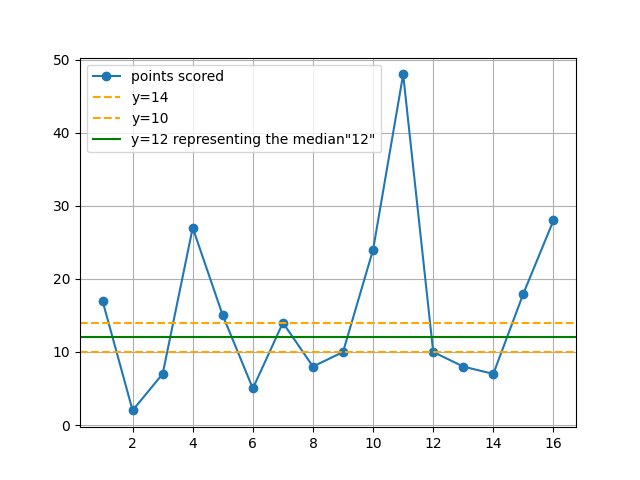
\includegraphics[scale=0.7]{Figure_12.png}
		\caption{Y-axis Illustrating different scores scored by a kabaddi team and X-axis shows match no. }
		\label{fig:1}
	\end{figure}
	
	
\end{document}